\onecolumn
\section*{Appendix}
% Your table in single-column mode
\begin{table}[h]
	\centering
	\begin{tabular}{rcccccccccc}
		                   & \texttt{Aves} & \texttt{Mammal} & \texttt{Reptile} & \texttt{Aerial} & \texttt{Aquatic} & \texttt{Terrestrial} & \texttt{Migratory} & \texttt{Solitary} & \texttt{Carnivore} & \texttt{Eggs} \\
		\hline
		\texttt{Bat}       &               & $\times$        &                  & $\times$        &                  &                      &                    &                   & $\times$           &               \\
		\texttt{Crocodile} &               &                 & $\times$         &                 & $\times$         & $\times$             &                    &                   & $\times$           & $\times$      \\
		\texttt{Crow}      & $\times$      &                 &                  & $\times$        &                  &                      &                    &                   &                    & $\times$      \\
		\texttt{Hippo}     &               & $\times$        &                  &                 & $\times$         & $\times$             &                    & $\times$          &                    &               \\
		\texttt{Ostrich}   & $\times$      &                 &                  &                 &                  & $\times$             &                    & $\times$          &                    & $\times$      \\
		\texttt{Penguin}   & $\times$      &                 &                  &                 & $\times$         & $\times$             & $\times$           &                   & $\times$           & $\times$      \\
		\texttt{Platypus}  &               & $\times$        &                  &                 & $\times$         & $\times$             &                    & $\times$          & $\times$           & $\times$      \\
		\texttt{Snake}     &               &                 & $\times$         &                 &                  & $\times$             &                    & $\times$          & $\times$           & $\times$      \\
		\texttt{Swallow}   & $\times$      &                 &                  & $\times$        &                  &                      & $\times$           & $\times$          & $\times$           & $\times$      \\
		\texttt{Whale}     &               & $\times$        &                  &                 & $\times$         &                      & $\times$           & $\times$          & $\times$           &               \\
	\end{tabular}
	\vspace{10pt}
	\caption{A formal context describing animals (objects) and some of their features (attributes)}
	\label{table: formal context}
\end{table}

\begin{figure}[b]
	\centering
	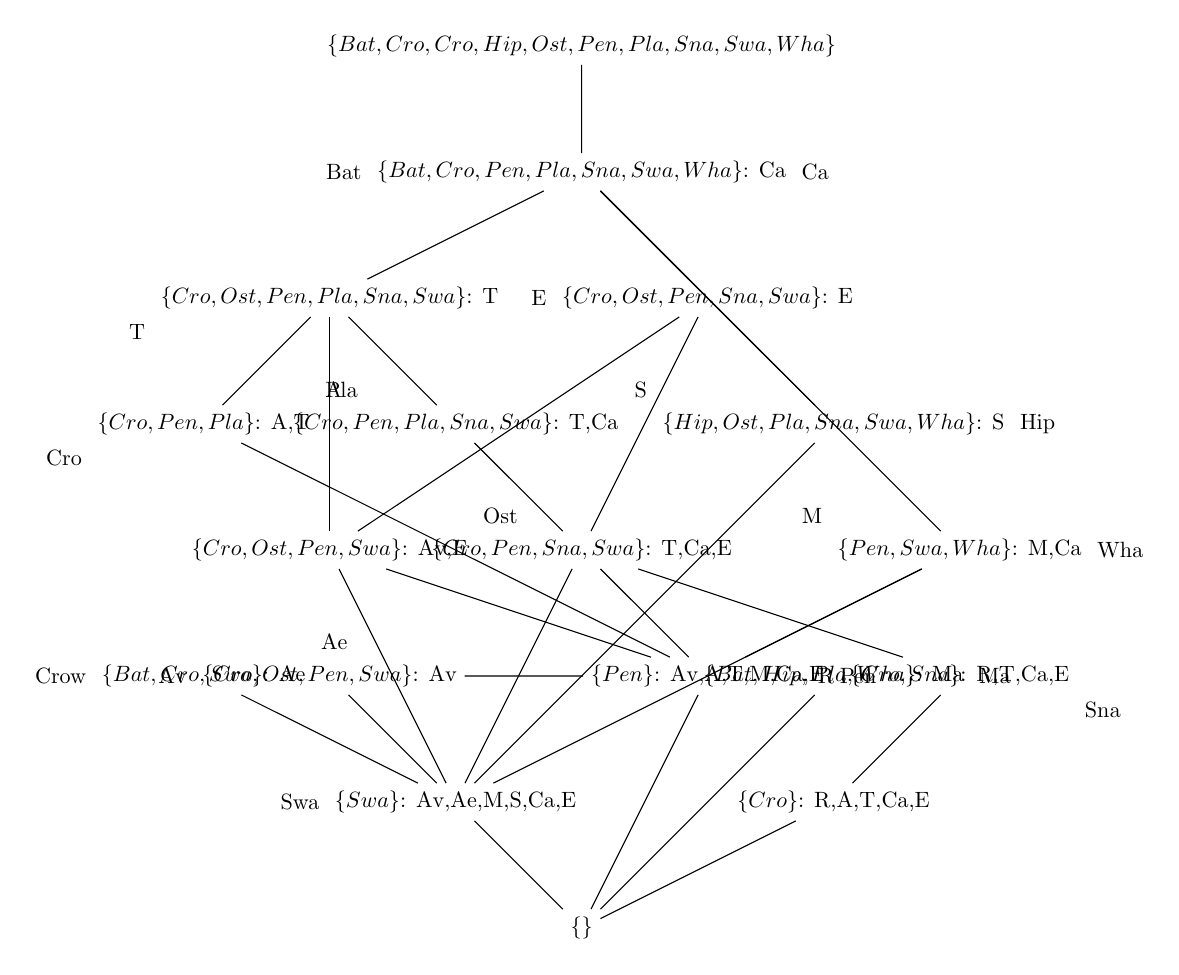
\begin{tikzpicture}[node distance=2cm, auto, scale=0.8, every node/.style={scale=0.8}]

		% Define the nodes
		\node (top) at (0,12) {$\{Bat,Cro,Cro,Hip,Ost,Pen,Pla,Sna,Swa,Wha\}$};
		\node (carnivore) at (0,10) {$\{Bat,Cro,Pen,Pla,Sna,Swa,Wha\}$: Ca};
		\node (terrestrial) at (-4,8) {$\{Cro,Ost,Pen,Pla,Sna,Swa\}$: T};
		\node (aquatic_terrestrial) at (-6,6) {$\{Cro,Pen,Pla\}$: A,T};
		\node (terrestrial_carnivore) at (-2,6) {$\{Cro,Pen,Pla,Sna,Swa\}$: T,Ca};
		\node (eggs) at (2,8) {$\{Cro,Ost,Pen,Sna,Swa\}$: E};
		\node (terrestrial_carnivore_eggs) at (0,4) {$\{Cro,Pen,Sna,Swa\}$: T,Ca,E};
		\node (solitary) at (4,6) {$\{Hip,Ost,Pla,Sna,Swa,Wha\}$: S};
		\node (migratory_carnivore) at (6,4) {$\{Pen,Swa,Wha\}$: M,Ca};
		\node (aerial) at (-6,2) {$\{Bat,Cro,Swa\}$: Ae};
		\node (swallow) at (-2,0) {$\{Swa\}$: Av,Ae,M,S,Ca,E};
		\node (aves) at (-4,2) {$\{Cro,Ost,Pen,Swa\}$: Av};
		\node (aves_eggs) at (-4,4) {$\{Cro,Ost,Pen,Swa\}$: Av,E};
		\node (penguin) at (2,2) {$\{Pen\}$: Av,A,T,M,Ca,E};
		\node (mammal) at (4,2) {$\{Bat,Hip,Pla,Wha\}$: Ma};
		\node (reptile_terrestrial_carnivore_eggs) at (6,2) {$\{Cro,Sna\}$: R,T,Ca,E};
		\node (crocodile) at (4,0) {$\{Cro\}$: R,A,T,Ca,E};
		\node (bottom) at (0,-2) {$\{\}$};

		% Define the edges
		\draw (top) -- (carnivore);
		\draw (carnivore) -- (terrestrial);
		\draw (carnivore) -- (eggs);
		\draw (carnivore) -- (solitary);
		\draw (carnivore) -- (migratory_carnivore);
		\draw (terrestrial) -- (aquatic_terrestrial);
		\draw (terrestrial) -- (terrestrial_carnivore);
		\draw (terrestrial) -- (aves_eggs);
		\draw (aquatic_terrestrial) -- (penguin);
		\draw (terrestrial_carnivore) -- (terrestrial_carnivore_eggs);
		\draw (eggs) -- (aves_eggs);
		\draw (eggs) -- (terrestrial_carnivore_eggs);
		\draw (terrestrial_carnivore_eggs) -- (swallow);
		\draw (terrestrial_carnivore_eggs) -- (penguin);
		\draw (terrestrial_carnivore_eggs) -- (reptile_terrestrial_carnivore_eggs);
		\draw (solitary) -- (swallow);
		\draw (migratory_carnivore) -- (swallow);
		\draw (migratory_carnivore) -- (penguin);
		\draw (aerial) -- (swallow);
		\draw (aves) -- (swallow);
		\draw (aves) -- (penguin);
		\draw (aves_eggs) -- (swallow);
		\draw (aves_eggs) -- (penguin);
		\draw (mammal) -- (bottom);
		\draw (reptile_terrestrial_carnivore_eggs) -- (crocodile);
		\draw (swallow) -- (bottom);
		\draw (penguin) -- (bottom);
		\draw (crocodile) -- (bottom);

		% Add labels for objects
		\node[left] at (carnivore.west) {Bat};
		\node[below left] at (aquatic_terrestrial.south west) {Cro};
		\node[left] at (aerial.west) {Crow};
		\node[right] at (solitary.east) {Hip};
		\node[above right] at (aves_eggs.north east) {Ost};
		\node[right] at (penguin.east) {Pen};
		\node[above right] at (aquatic_terrestrial.north east) {Pla};
		\node[below right] at (reptile_terrestrial_carnivore_eggs.south east) {Sna};
		\node[left] at (swallow.west) {Swa};
		\node[right] at (migratory_carnivore.east) {Wha};

		% Add labels for attributes
		\node[above right] at (aerial.north east) {Ae};
		\node[left] at (aves.west) {Av};
		\node[right] at (carnivore.east) {Ca};
		\node[left] at (eggs.west) {E};
		\node[right] at (mammal.east) {Ma};
		\node[above left] at (migratory_carnivore.north west) {M};
		\node[left] at (reptile_terrestrial_carnivore_eggs.west) {R};
		\node[above left] at (solitary.north west) {S};
		\node[below left] at (terrestrial.south west) {T};
		\node[above right] at (aquatic_terrestrial.north east) {A};

	\end{tikzpicture}
	\caption{Concept Lattice for Animal Attributes}
	\label{fig:animal-concept-lattice}
\end{figure}

\twocolumn

% \begin{table}
%     \centering
%     \begin{tabular}{r|c|c|c|c|c|c|c|c|c|c}
%                            & \texttt{Aves} & \texttt{Mammal} & \texttt{Reptile} & \texttt{Aerial} & \texttt{Aquatic} & \texttt{Terrestrial} & \texttt{Migratory} & \texttt{Solitary} & \texttt{Carnivore} & \texttt{Eggs} \\
%         \hline
%         \texttt{Bat}       &               & $\times$        &                  & $\times$        &                  &                      &                    &                   & $\times$           &               \\
%         \texttt{Crocodile} &               &                 & $\times$         &                 & $\times$         & $\times$             &                    &                   & $\times$           & $\times$      \\
%         \texttt{Crow}      & $\times$      &                 &                  & $\times$        &                  &                      &                    &                   &                    & $\times$      \\
%         \texttt{Hippo}     &               & $\times$        &                  &                 & $\times$         & $\times$             &                    & $\times$          &                    &               \\
%         \texttt{Ostrich}   & $\times$      &                 &                  &                 &                  & $\times$             &                    & $\times$          &                    & $\times$      \\
%         \texttt{Penguin}   & $\times$      &                 &                  &                 & $\times$         & $\times$             & $\times$           &                   & $\times$           & $\times$      \\
%         \texttt{Platypus}  &               & $\times$        &                  &                 & $\times$         & $\times$             &                    & $\times$          & $\times$           & $\times$      \\
%         \texttt{Snake}     &               &                 & $\times$         &                 &                  & $\times$             &                    & $\times$          & $\times$           & $\times$      \\
%         \texttt{Swallow}   & $\times$      &                 &                  & $\times$        &                  &                      & $\times$           & $\times$          & $\times$           & $\times$      \\
%         \texttt{Whale}     &               & $\times$        &                  &                 & $\times$         &                      & $\times$           & $\times$          & $\times$           &               \\
%     \end{tabular}
%     \caption{Cross-table of $\K$}
%     \label{tab:formal-context}
% \end{table}


\begin{algorithm}
	\caption{Computing the tolerance partition on objects $G$}
	\begin{algorithmic}[1]
		\Require A formal context, $\FC$;
		\Require A set of defeasible implications, $\Delta$;
		\Ensure A tolerance partition $(R_0, \ldots, R_n)$ on $G$;
		\State $P_0 \gets G$;
		\State $i \gets 0$;
		\State $\Delta \gets \text{Material} (\Delta)$;
		\While {$P_{i-1} \neq P_i}$
			\State $P_{i+1} \gets \{g \in P_i \mid \exists \delta \in \Delta  g' \st g'\not \models \delta \}$;
			\State $R_i \gets P_i \setminus P_{i+1}$;
			\State $\Delta_i \gets \{ (\alpha \rightarrow \beta) \in \Delta \mid \exists g \in P_i \st \alpha \subseteq g'\}$;
			\State $\Delta \gets \Delta \setminus \Delta_i$;
			\EndWhile
			\If {$P_{i-1} = \emptyset$}
			\State $n \gets i-1$;
			\Else
			\State $n \gets i$;
			\EndIf
			\State \Return $\big (R_0,\ldots, R_n \big)$;
	\end{algorithmic}
\end{algorithm}

To clarify some points on
\begin{itemize}
	\item Line $3$: this step turns $\Delta$ into a set of material implications;
	\item Line $5$: this step puts into ranking $i+1$ every object which \textbf{does not} respect $\Delta$;
	\item Line $7$: this sets $\Delta_i$ to be the set of formulae in $\Delta$ which have their antecedent satisfied by an object in $P_i$ (implicitly all objects in $P_i$ satisfy all formulae in $\Delta$, but we only care about the ones which have their antecedent satisfied);
	\item We update $\Delta$ to be those formulae which are not yet ``dealt with''.
\end{itemize}

\begin{algorithm}
	\caption{Checking entailment}
	\begin{algorithmic}[1]
		\Require A formal context, $\FC$;
		\Require A set of defeasible implications, $\Delta$;
		\Ensure A tolerance partition $(R_0, \ldots, R_n)$ on $G$;
		\State $P_0 \gets G$;
		\State $i \gets 0$;
		\State $\Delta \gets \text{Material} (\Delta)$;
		\While {$P_{i-1} \neq P_i}$
			\State $P_{i+1} \gets \{g \in P_i \mid \exists \delta \in \Delta  g' \st \not \Vdash \delta \}$;
			\State $P_i \gets P_i \setminus P_{i+1}$;
			\State $\Delta_i \gets \{ (\alpha \rightarrow \beta) \in \Delta \mid \exists g \in P_i \st \alpha \subseteq g'\}$;
			\State $\Delta \gets \Delta \setminus \Delta_i$;
			\EndWhile
			\If {$P_{i-1} = \emptyset$}
			\State $n \gets i-1$;
			\Else
			\State $n \gets i$;
			\EndIf
			\State \Return $\big (P_0,\ldots, P_n \big)$;
	\end{algorithmic}
\end{algorithm}